\documentclass[10pt,journal]{IEEEtran}  %10pt, sans, memo

\usepackage{subcaption}
\usepackage{amsthm}

\usepackage[utf8]{inputenc}

\usepackage{tikz}
\usepackage{tikzscale}
\usepackage{pgfplots}

\usepackage{booktabs}
\usepackage{graphicx}
\usepackage{mathtools}
\usepackage{breqn}
\usepackage{natbib}

\usepackage{hyperref}

\bibliographystyle{ieeetr} 

\author{Jonathan Dyer}
\date{\today}
\title{High Resolution Space-based Remote Sensing Trade Space}
\hypersetup{
 pdfauthor={Jonathan Dyer},
 pdftitle={EO Modalities},
 pdfkeywords={},
 pdfsubject={},
 pdfcreator={}, 
 pdflang={English}}

\newcommand{\includepgf}[3]
{
  \begin{figure}[h!]
  \centering
  \includegraphics{#1}
  \caption[]{#3}
  \label{#2}
  \end{figure}
}

\DeclarePairedDelimiter{\abs}{\lvert}{\rvert}
\DeclarePairedDelimiter{\norm}{\lVert}{\rVert}

\begin{document}

\newtheorem{mydef}{Definition}

\makeatletter
\newcommand\footnoteref[1]{\protected@xdef\@thefnmark{\ref{#1}}\@footnotemark}
\makeatother

\author{Jonathan~Dyer,~\IEEEmembership{Member,~IEEE,}
        Dirk~Robinson,~\IEEEmembership{Member,~IEEE,}
        and~Paul~Boerner,~\IEEEmembership{Member,~IEEE}%
}

\markboth{Journal of \LaTeX\ Class Files,~Vol.~14, No.~8, August~2015}%
{}
        
        
\IEEEtitleabstractindextext{%
\begin{abstract}
The abstract goes here.
\end{abstract}


% Note that keywords are not normally used for peerreview papers.
\begin{IEEEkeywords}
IEEE, remote sensing, satellite, spacecraft, high resolution.
\end{IEEEkeywords}}


% make the title area
\maketitle

\IEEEdisplaynontitleabstractindextext

\section{Introduction}
\label{sec:introduction}

The trade space for high resolution remote sensing spacecraft is nuanced and many assumptions made historically in the architecture of such systems are less valid in light of rapid developments in image sensors, attitude control and other spacecraft subsystems.  In this article, we explore the trade space specifically in light of the recent trend toward smaller, lower cost spacecraft.

\section{Performance Trade Space}
\label{sec:trade_space}

The high resolution imaging trade space is fairly well constrained by a few driving requirements which are, in turn, driven by four primary mission needs:

\begin{enumerate}
\item Phenomenology
\item Image Quality
\item Collection Capacity
\item Cost
\end{enumerate}

\emph{Phenomenology} refers to the phenomenon being sensed or study and drives things like the spectral range, signal-to-noise ratio (SNR) and resolution required.  

\emph{Image Quality}, likewise, drives resolution and SNR.  

\emph{Collection capacity} drives many system variables both within the payload (such as swath width) as well as elsewhere in the spacecraft (collection rate, attitude control agility).  

\emph{Cost} is an increasingly important constraint placed on both technology selection and physical dimensions of the spacecraft.

We will spend significant time studying the system trades impacting Image Quality, Collection Capacity and Cost.  Phenomenology will only be addressed in passing.

\section{Remote Sensing Driving Requirements}
\label{sec:requirements}

Taken together these mission needs define the requirement trade space we will study here.  In order to facilitate discussion of these system trades, we will define some key system performance metrics in the following sections but first we will introduce the non-dimensional parameter $Q$.

\subsection{$\frac{\lambda F^\#}{p}$ or Q}
\label{sec:q}

The system parameter $Q$ is defined as:

\begin{equation}
Q = \frac{\lambda F^\#}{p}
\label{eq:Q}
\end{equation}
and is essentially a measure pixel sampling in the spatial domain relative to the Nyquist criterion.  Nyquist says that to completely reconstruct a band-limited system, the spatial sampling frequency. 
$$\rho_s = 1/p \geq 2 BW_{opt}$$

Because we always sample to DC, the optical bandwidth $BW_{opt}$ is replaced by the diffraction cutoff frequency.
$$\rho_c = \frac{1}{\lambda F^\#}$$

Thus $Q$ is a measure of Nyquist sampling where $Q=2$ is critically sampled.  Most systems, however, operate at $Q < 2$ and hence incur some spatial aliasing.  There is little reason to operate at $Q > 2$ as the optics do not pass spatial frequency information there so the additional sampling is essentially wasted.

\begin{figure}[h!]
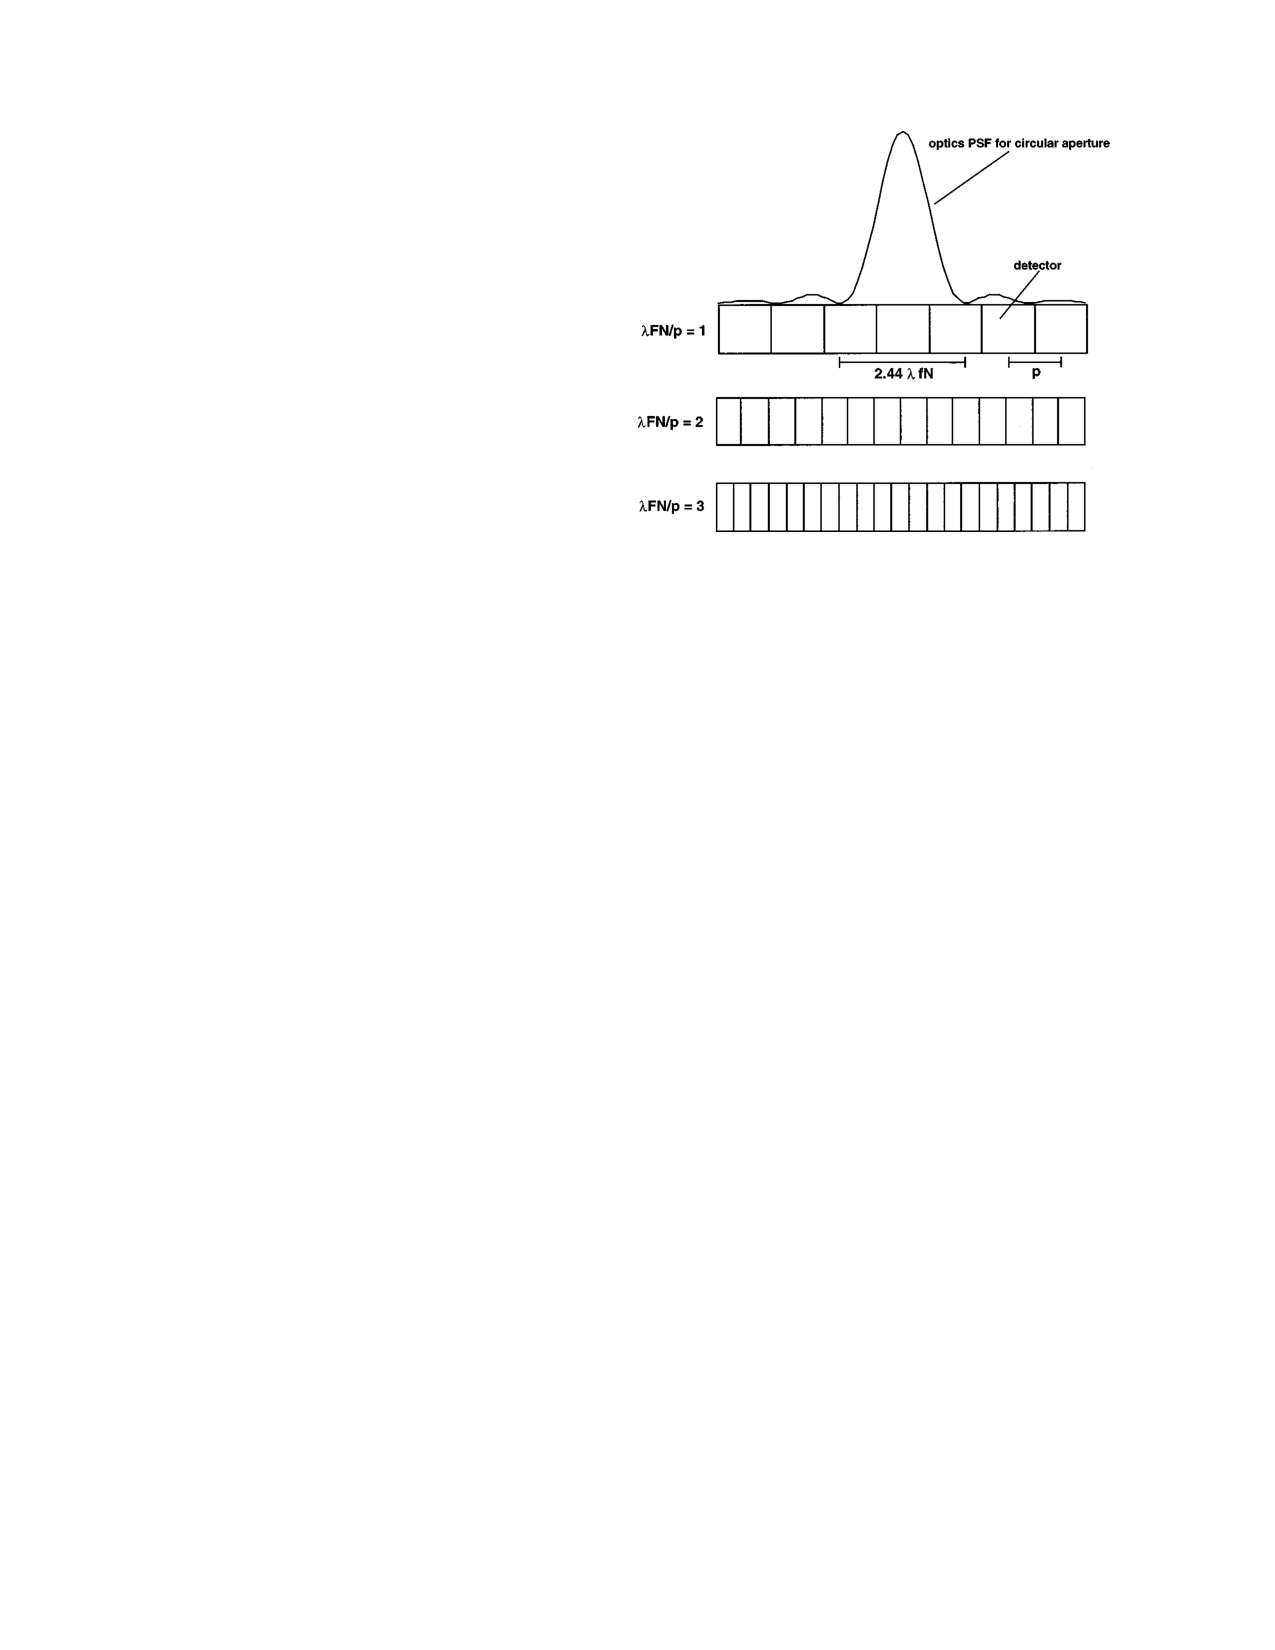
\includegraphics[width=0.42\textwidth]{figures/Q_fiete.pdf}
\caption{Spatial interpretation of Q sampling a diffraction-limited PSF.  Adapted from \cite{fiete_q})}
\end{figure}

In section \ref{sec:image_quality} we will argue that from an image quality perspective it is desirable to have $1.2 < Q < 1.6$ for typical high-resolution remote sensing systems.  

Beyond a statement of the Nyquist criterion, $Q$ is a very useful parameter by which to evaluate and compare systems.  For more see \cite{fiete_q}.  $Q$ will be used regularly throughout this memo.

\subsection{Resolution}
Resolution is a surprisingly difficult-to-define metric.  Often Ground Sample Distance (GSD) is used as a proxy for resolution under the [implicit] assumption that all pixels are created equally.  This assumption doesn't hold for systems with widely varying SNR or sharpness (see Section \ref{sec:q}).

More wholistic definitions of resolution typically refer back to \emph{resolvability} or the ability to distinguish objects or features of a given size in an image.  The so-called Ground Resolution Distance (GRD) is an example of a such a metric.  Unfortunately the definition of GRD is not universally agreed to or consistent.  We will use the definition of GRD proposed in \cite{auelmann_iq} where:

\begin{equation}
    \alpha_{eff} = \frac{IFOV}{RER} = \frac{\lambda_{mean}}{D\times Q \times RER}
\label{eq:alpha_eff}
\end{equation}

\cite{auelmann_iq} has shown that a good approximation for $\alpha_{eff}$ for diffraction limited systems is given by:


\begin{equation}
    \alpha_{eff} \approx \frac{\lambda_{mean}}{D}\left[1 + \frac{1}{Q^{1.35}}\right]^{1/1.35}
\label{eq:alpha_eff_approx}
\end{equation}

\includepgf{figures/resolution_q.pgf}{fig:resolution_q}{Relationship of GRD and GSD as resolution metrics as a function of Q}

Notice in Figure \ref{fig:resolution_q} that GRD asymptotes at $Q=2$ but that GSD continues decreasing monotonically.  This is due to the fact that optical systems do not pass spatial frequency beyond the diffraciton limit which is critically sampled at $Q=2$ and illustrates why GSD-alone is a problematic resolution metric.

\subsection{Dynamic Range (DR) and Signal-to-noise Ratio}
Dynamic range and signal-to-noise ratio are closely related by subtedly different measures of radiometric performance.

Dynamic range is defined as the ratio of maximum-to-minimum signal level that the system can capture or represent in an image:

\begin{equation}
DR = \frac{S_{max}}{S_{min}}
\label{eq:DR}
\end{equation}

The minimum signal level is the noise-floor of the system, $S_{min} = \sigma$ where $\sigma$ represents all non-signal-correlated noise sources in the system including read noise, dark current, etc.

The maximum signal is the maximum number of photo-electrons the system can capture for one output image pixel and is limited by the well depth of a pixel, $S_{max} = N_{e^-}^{well}$ for single-exposure systems.  Note that in digitally oversampled systems (covered later), the digital oversampling factor directlye expands dynamic range by increasing the effective well depth such that $S_{max} = N_f N_{e^-}^{well}$ where $N_f$ is the oversampling ratio.  Oversampling also affects $S_{min}$ and it can be shown that, for equally exposed samples:

\begin{equation}
    DR = \sqrt{N_f}\frac{N_{e^-}^{well}}{\sigma}
\label{eq:DR_OS}
\end{equation}

For systems that digitally oversample with unequal exposures, the dynamic range can be even larger as is shown in section TBD.

Signal-to-noise ratio, like dynamic range, depends critically on both the detector well depth and its noise characteristics.  

\subsubsection{Data Intensity}

\subsubsection{Detector Capture Rate}

\subsubsection{Collection Rate}

\subsubsection{Optical Complexity}

captured in Table \ref{table:drivers}.

\begin{table}[h!t]
\resizebox{.45\textwidth}{!}{%
\begin{tabular}{@{}ll@{}}
\toprule
\textbf{Requirement} & \textbf{Drives} \\ \toprule
Resolution & \begin{tabular}[c]{@{}l@{}}Aperture Diameter\\ Altitude\end{tabular} \\ \midrule
\begin{tabular}[c]{@{}l@{}}SNR \& Dynamic Range\end{tabular} & \begin{tabular}[c]{@{}l@{}}Stabilization\\ Detector Full-well\\Optical $F^\#$\end{tabular} \\ \midrule
Swath Width & \begin{tabular}[c]{@{}l@{}}Optical Complexity\\ Detector Width\\ Data Volume\end{tabular} \\ \midrule
Collection Rate & \begin{tabular}[c]{@{}l@{}}Stabilization\\ Detector capture rate\end{tabular} \\ \midrule
Spectral Sampling & \begin{tabular}[c]{@{}l@{}}In-track FOV\\ Camera filters\\ Semiconductor Bandgap\end{tabular} \\ \bottomrule
\end{tabular}%
}
\centering
\caption{System Performance Drivers}
\label{table:drivers}
\end{table}

It is important to note that many of these requirements are tightly coupled.  For example chosing a high resolution requirement directly impacts the difficulty of meeting other requirements:

\begin{itemize}
\item High resolution drives either a reduction in achievable SNR or a increase in required integration time and associated tighter ACS stability and more powerful image stabilization
\item Recovering SNR at high resolution drives detectors with high read-out (for digital oversampling) and/or significant analogy stabilization (TDI or optical)
\item High resolution increases focal plane width and data intensity or reduces swath width while still increasing data intensity

\end{itemize}

\subsection{Image Quality}
\label{sec:iq}

Image quality is a complex, multi-faceted subject and while there is no perfect model or metric, substantial work has gone into quantifying the image quality of high resolution remote sensing systems.  High resolution systems are typically evaluated by quantitative "image interpretability" scales the best known being the National Image Interpretability Rating Scale, or NIIRS.

NIIRS rating is described by specific human interpretation standards, examples of which are shown in Table \ref{table:NIIRS}\cite{niirs}.

\begin{table}[h!b]
\resizebox{.45\textwidth}{!}{%
\begin{tabular}{@{}lll@{}}
\toprule
\textbf{NIIRS} & \textbf{GRD}          & \textbf{Description}                                                                                                                             \\ \toprule
3     & 2.5m - 4.5m  & \begin{tabular}[c]{@{}l@{}}Identify a road as divided or undivided\\ Detect rows of automobiles in a parking lot\end{tabular}           \\ \midrule
4     & 1.2m - 2.5m  & \begin{tabular}[c]{@{}l@{}}Detect barriers/obstacles (barrels) on runways\\ Distinguish between locomotives and railcars\end{tabular}   \\ \midrule
5     & 0.75m - 1.2m & \begin{tabular}[c]{@{}l@{}}Identify individual lines painted on paved roads,  parking lots\\ Identify fallen utility poles\end{tabular} \\ \midrule
6     & 0.4m - 0.75m & \begin{tabular}[c]{@{}l@{}}Detect individuals, when not in a group\\ Detect small road signs in an urban area\end{tabular}              \\ \bottomrule
\end{tabular}%
}
\centering
\caption{NIIRS definitions}
\label{table:NIIRS}
\end{table}

Note that $GRD$ stands for Ground Resolving Distance and is NOT the same as $GSD$.  There are various formal definitions for $GRD$ but it is essentially the minimum resolvable detail in the image which depends on $GSD$, sharpness or edge response and $SNR$.

NIIRS is a logarithmic scale traditionally evaluated by trained human image interpreters.  However, much work has gone into developing semi-analytic regressions to predict NIIRS from basic image quality parameters such as sharpness, signal-to-noise ratio (SNR), etc. The Generalized Image Quality Equation (GIQE) is an example of such a function; we will use the 5th version, GIQE-5 which is defined in eq. \ref{eq:giqe5}.

\begin{dmath}
NIIRS = 4.4 - 3.32 \log(GSD_{m}) + 3.32 \left[1 - e^{\frac{-5.308}{\Delta SNR}}\right]\log(RER_0)
- 0.402 \log(RER_0)^4 - 2.92/\Delta SNR - 0.069N_{smear}
\label{eq:giqe5}
\end{dmath}
where $GSD_{m}$\footnote{GSD units must be paid close attention to - many references list GIQE using units of inches for GSD.  In this case, the first parameter in the equation is 9.7 rather than 4.4 because $4.4 - 3.32\log{\left(39.4 \frac{in}{m}\right)} \approx 9.7$} is the ground sample distance in meters, $\Delta SNR$ is difference between $SNR$ for a 15\% and 8\% target reflectance, $RER_0$ is the raw Relative Edge Response (without sharpening or MTFC) and $N_{smear}$ is the number of pixels of linear smear.

GIQE-5 is fairly well validated again human interpreters \cite{giqe5} and nicely captures the trade-off between various imaging system parameters such as $SNR$ and $GSD$.  One thing noticed in parametric study of the GIQE-5 is that image quality is often maximized at $Q>1$ (Fig. \ref{fig:sq_iq}).  This has also been validated in human-interpreter studies \cite{fiete_Q_IQ} which indicate that $Q \sim 1.5$ is the optimal balance of resolution and $SNR$ for most real space-based high resolution systems.  
\subsubsection{Resolution}

\subsubsection{Signal-to-noise Ratio (SNR) and Dynamic Range (DR)}

\subsubsection{NIIRS}

\subsection{Collection Capacity}
\label{sec:capacity}

\subsubsection{Swath Width}

\subsubsection{Scanrate and Blur}

\subsubsection{Data Intensity}

\subsection{Cost}
\label{sec:cost}

\subsubsection{Dimension}

\subsubsection{Sub-system requirements}

\subsubsection{Complexity}

\section{Imaging Modalities}
\label{sec:modalities}

\subsection{Background and Definition for Analyses}
\label{sec:analyses_background}

\subsubsection{Photon radiometry}

\subsection{Time-delayed Integration (TDI)}
\label{sec:tdi}

\subsection{Step-and-Stare}
\label{sec:step_stare}

\subsection{Stabilized Step-and-Stare}
\label{sec:stab_step_stare}

\subsection{Comparison of Modalities}
\label{sec:comp_modalities}

\section{Example Systems}
\label{sec:examples}

\subsection{Medium Resolution Small Satellite}
\label{sec:med_res}

\subsection{High Resolution Small Satellite}
\label{sec:high_res}

\subsection{Very-high Resolution Small Satellite}
\label{sec:vhigh_res}

\section{Conclusions}
\label{sec:conclusions}

\bibliography{main}

\end{document}
